
%(BEGIN_QUESTION)
% Copyright 2006, Tony R. Kuphaldt, released under the Creative Commons Attribution License (v 1.0)
% This means you may do almost anything with this work of mine, so long as you give me proper credit

Examine the following loop diagram:

$$\includegraphics[width=15.5cm]{i00136x01.eps}$$

Trace the path of current in the signal wiring, then determine the following voltage drops at the respective flow rates.  Assume a power supply voltage of exactly 24 volts DC:

\begin{itemize}
\item{} Voltage across FY-14 resistor = \underbar{\hskip 50pt} ; Flow rate = 100 GPM
\item{} Voltage between terminals TB40-3 and TB40-4 = \underbar{\hskip 50pt} ; Flow rate = 200 GPM
\item{} Voltage across FT-14 transmitter terminals = \underbar{\hskip 50pt} ; Flow rate = 175 GPM
\item{} Voltage between terminals TB64-8 and TB27-15 = \underbar{\hskip 50pt} ; Flow rate = 200 GPM
\end{itemize}

\underbar{file i00136}
%(END_QUESTION)





%(BEGIN_ANSWER)

$$\includegraphics[width=15.5cm]{i00136x02.eps}$$

\noindent
{\bf Partial answer:}

\begin{itemize}
\item{} Voltage across FY-14 resistor = \underbar{\bf 2.6 volts} ; Flow rate = 100 GPM
\item{} Voltage between terminals TB40-3 and TB40-4 = \underbar{\bf 19.8 volts} ; Flow rate = 200 GPM
\item{} Voltage across FT-14 transmitter terminals = \underbar{\hskip 50pt} ; Flow rate = 175 GPM
\item{} Voltage between terminals TB64-8 and TB27-15 = \underbar{\hskip 50pt} ; Flow rate = 200 GPM
\end{itemize}

%(END_ANSWER)





%(BEGIN_NOTES)

\begin{itemize}
\item{} Voltage across FY-14 resistor = \underbar{\bf 2.6 volts} ; Flow rate = 100 GPM
\item{} Voltage between terminals TB40-3 and TB40-4 = \underbar{\bf 19.8 volts} ; Flow rate = 200 GPM
\item{} Voltage across FT-14 transmitter terminals = \underbar{\bf 20.2 volts} ; Flow rate = 175 GPM
\item{} Voltage between terminals TB64-8 and TB27-15 = \underbar{\bf 0 volts} ; Flow rate = 200 GPM
\end{itemize}

\vskip 20pt \vbox{\hrule \hbox{\strut \vrule{} {\bf Virtual Troubleshooting} \vrule} \hrule}

This question is a good candidate for a ``Virtual Troubleshooting'' exercise.  Presenting the diagram to students, you first imagine in your own mind a particular fault in the system.  Then, you present one or more symptoms of that fault (something noticeable by an operator or other user of the system).  Students then propose various diagnostic tests to perform on this system to identify the nature and location of the fault, as though they were technicians trying to troubleshoot the problem.  Your job is to tell them what the result(s) would be for each of the proposed diagnostic tests, documenting those results where all the students can see.

During and after the exercise, it is good to ask students follow-up questions such as:

\begin{itemize}
\item{} What does the result of the last diagnostic test tell you about the fault?
\item{} Suppose the results of the last diagnostic test were different.  What then would that result tell you about the fault?
\item{} Is the last diagnostic test the best one we could do?
\item{} What would be the ideal order of tests, to diagnose the problem in as few steps as possible?
\end{itemize}

%INDEX% Basics, loop-powered transmitter: voltage drop calculations
%INDEX% Documentation, loop diagram

%(END_NOTES)


